\section{Практическая часть}

\noindent\textbf{Начальные условия.}
В работе используется прямоугольный волновод размерами $23 \times 10$~мм. Шаг перемещения зонда и антенны при снятии экспериментальных зависимостей составляет $3$~мм. Расстояние от антенны до отражающего щита
\begin{equation}
	X = 283~\text{см} = 2{,}83~\text{м}.
\end{equation}

\noindent\textbf{Проверка применимости метода.}
Убедимся, что щит находится в зоне Фраунгофера:
\begin{equation}
	X \gg \frac{\max\{l_1^2, l_2^2\}}{\lambda}
	= \frac{187{,}69~\text{см}^2}{3{,}3~\text{см}}
	\approx 57~\text{см},
\end{equation}
то есть условие выполняется.

\subsection{Задание 1. Поле при отсутствии принимаемого сигнала}

Перед антенной помещается щит с поглощающим покрытием, позволяя не учитывать отражённую от металлического щита часть поля. Была снята зависимость интенсивности электрического поля $|E|^2$ от координаты внутри волновода $x$. Полученная зависимость приведена на \cref{fig:graph:1}, исходные данные~--- в \cref{tab:practice1}.

При отсутствии отражённой компоненты уравнение \cref{eq:th:13} упрощается к виду
\begin{equation}
	|E|^2 \approx 1 + 2\Gamma_\kappa \cos(2hx + \varphi_\kappa).
	\label{eq:pr:1.1}
\end{equation}

Отсюда по полученной зависимости $|E|^2(x)$ можно определить коэффициент $\Gamma_\kappa$:
\begin{equation}
	\Gamma_\kappa
	= \frac{|E_{\max}|^2 - |E_{\min}|^2}{2\bigl(|E_{\max}|^2 + |E_{\min}|^2\bigr)}
	= \frac{|54|^2 - |45|^2}{2\bigl(|54|^2 + |45|^2\bigr)}
	= \frac{2916 - 2025}{2(2916 + 2025)}
	= \frac{891}{9882}
	\approx 0{,}026.
	\label{eq:pr:1.2}
\end{equation}

\begin{figure}[H]
	\centering
	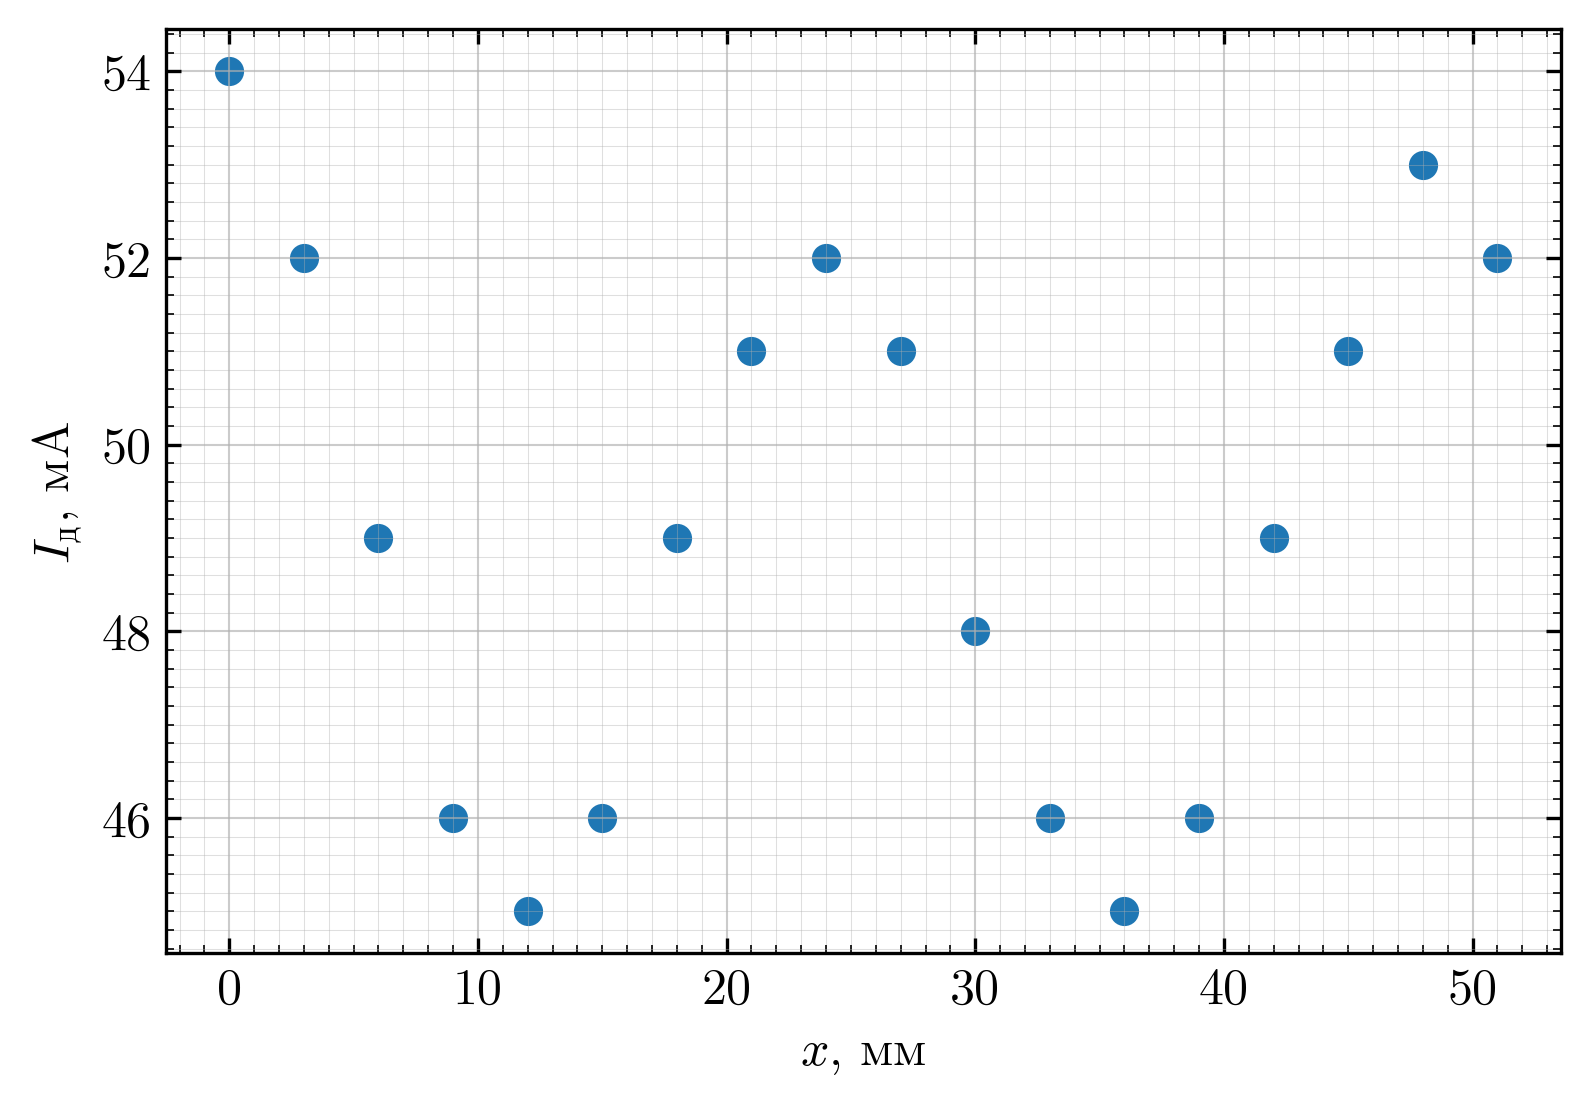
\includegraphics[width=0.7\linewidth]{graph/Figure_1}
	\caption{}
	\label{fig:graph:1}
\end{figure}


\noindent\textbf{Определение длины волны в волноводе.}
По \cref{tab:practice1} видно, что минимумы показаний располагаются при $x_1 = 12$~мм и $x_2 = 36$~мм, а расстояние между соседними минимумами равно
\begin{equation}
	\frac{\lambda_{\text{в}}}{2} = x_2 - x_1 = 36 - 12 = 24~\text{мм}.
\end{equation}
Следовательно,
\begin{equation}
	\lambda_{\text{в}} = 2 \cdot 24 = 48~\text{мм} = 4{,}8~\text{см}.
\end{equation}

Длина волны в свободном пространстве связана с длиной волны в волноводе соотношением
\begin{equation}
	\lambda_{\text{в}} = \frac{\lambda}{\sqrt{1 - \dfrac{a^2}{b^2}}},
\end{equation}
где $a$ и $b$~--- размеры поперечного сечения волновода. Отсюда
\begin{equation}
	\lambda = \lambda_{\text{в}} \sqrt{1 - \frac{a^2}{b^2}}.
\end{equation}

При частоте генератора $9{,}5$~ГГц свободная длина волны по номинальной частоте равна примерно $31{,}6$~мм, поэтому полученное значение $\lambda_{\text{в}} = 48$~мм отличается от расчётного примерно на $5\%$. Такое расхождение может быть связано с дискретностью шага, определением координат экстремумов и погрешностью отсчёта показаний.

Так как детектор квадратичный, коэффициент бегущей волны необходимо вычислять через корень из отношения показаний:
\begin{equation}
	\kappa_{\text{к}} = \frac{E_{\min}}{E_{\max}} = \sqrt{\frac{I_{\min}}{I_{\max}}}
	= \sqrt{\frac{45}{54}}
	\approx 0{,}9129.
\end{equation}

Коэффициент отражения от конца волноводного тракта:
\begin{equation}
	\Gamma_{\text{к}} = \frac{1 - \kappa_{\text{к}}}{1 + \kappa_{\text{к}}}
	= \frac{1 - 0{,}9129}{1 + 0{,}9129}
	\approx 0{,}0455.
\end{equation}

Соответствующий этому отражению коэффициент передачи по мощности (оценка потерь только за счёт рассогласования):
\begin{equation}
	\eta_{\text{согл}} = 1 - \Gamma_{\text{к}}^2
	= 1 - 0{,}0455^2
	= 1 - 0{,}0021
	\approx 0{,}9979
	= 99{,}79\%.
\end{equation}

Для второго задания необходимо установить координату, при которой
\begin{equation}
	\cos(2hx + \varphi_{\text{к}}) = 0.
\end{equation}
Из экспериментальной зависимости можно взять соседние экстремумы при $x = 24$~мм и $x = 36$~мм. Тогда
\begin{equation}
	X_0 = \frac{24 + 36}{2} = \frac{60}{2} = 30~\text{мм}.
\end{equation}

\subsection{Задание 2. Определение КНД по изменению расстояния до щита}

После удаления щита с поглощающим покрытием антенна перемещалась относительно металлического щита, а измерительная линия оставалась в положении $X_0 = 30$~мм. Результаты измерений приведены в \cref{tab:practice2}, графическая зависимость~--- на \cref{fig:graph:2}.
\begin{figure}[H]
	\centering
	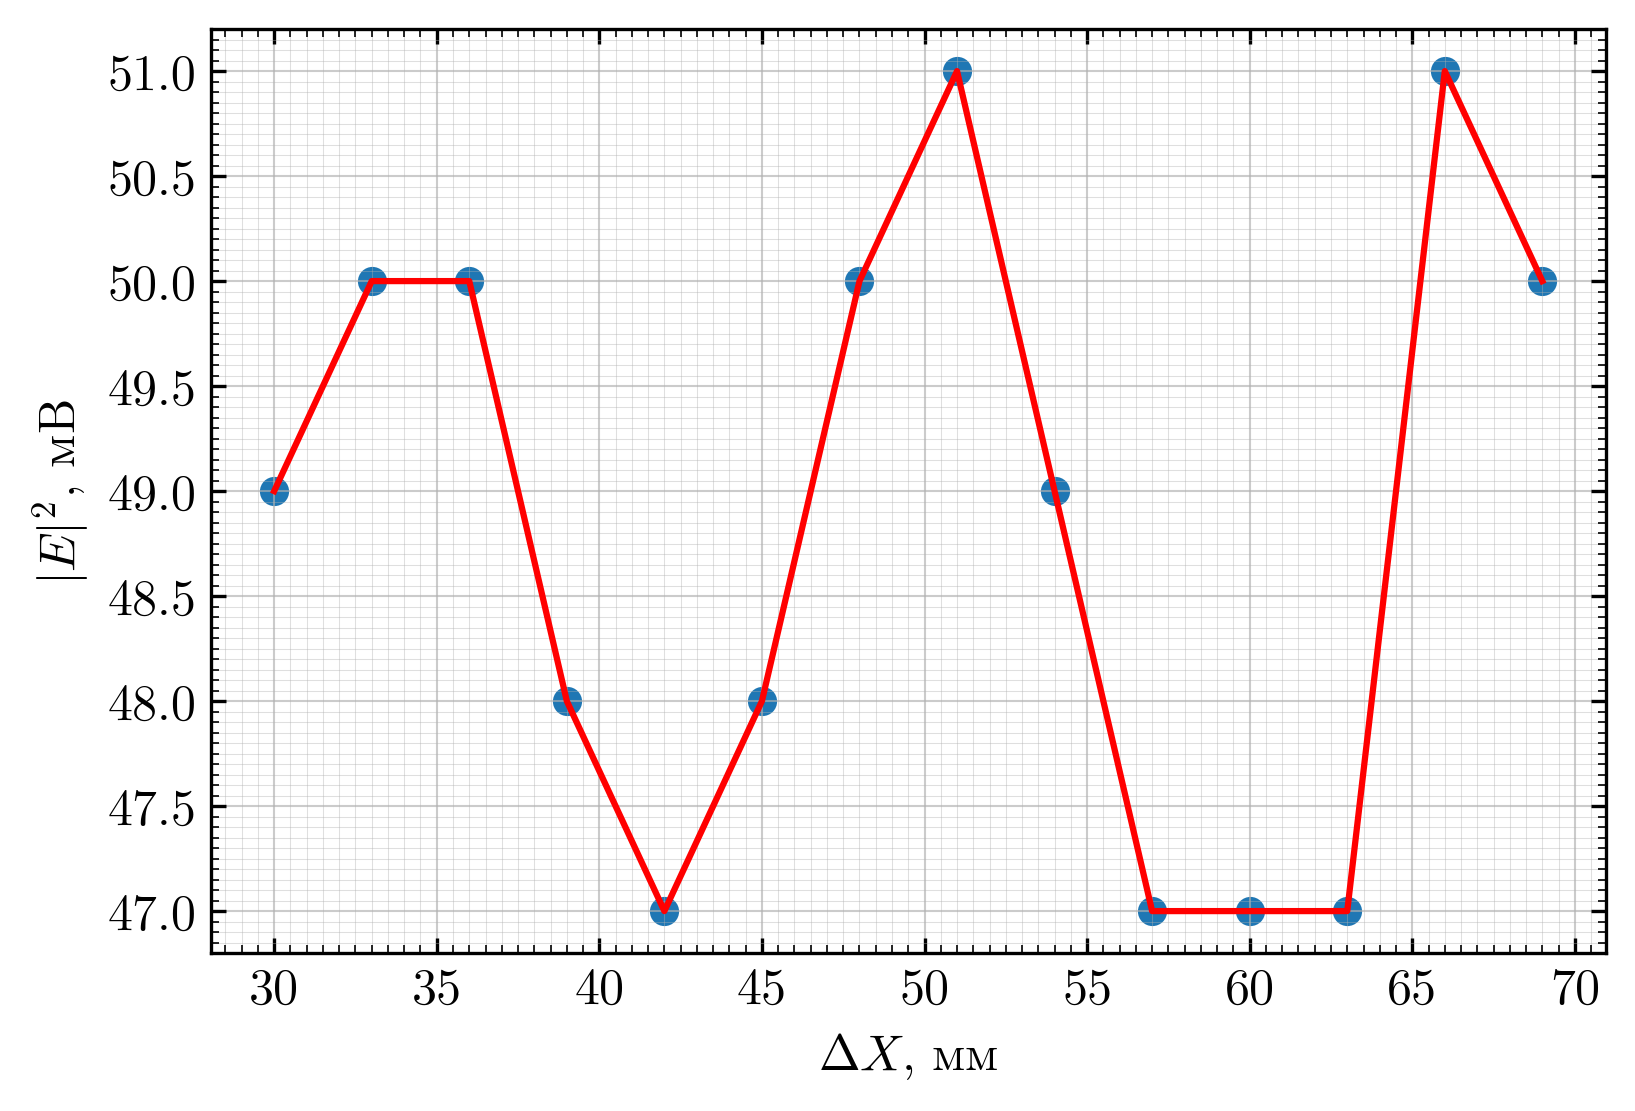
\includegraphics[width=0.7\linewidth]{graph/Figure_2}
	\caption{}
	\label{fig:graph:2}
\end{figure}
Максимальное и минимальное показания детектора составили
\begin{equation}
	I_{\max} = 51~\text{мА}, \qquad I_{\min} = 47~\text{мА}.
\end{equation}

Так как детектор квадратичный, коэффициент отражения от металлического щита можно оценить по амплитудам:
\begin{equation}
	\Gamma_2 = \frac{\sqrt{I_{\max}} - \sqrt{I_{\min}}}{\sqrt{I_{\max}} + \sqrt{I_{\min}}}
	= \frac{\sqrt{51} - \sqrt{47}}{\sqrt{51} + \sqrt{47}}
	\approx 0{,}0204.
	\label{eq:pr:2.1}
\end{equation}

Используя формулу~(14)
\begin{equation}
	D = \frac{8\pi X}{\lambda}\Gamma,
\end{equation}
получаем
\begin{equation}
	D_2 = \frac{8\pi X}{\lambda}\Gamma_2
	= \frac{8\pi \cdot 2{,}83}{0{,}03321} \cdot 0{,}0204
	\approx 43{,}7,
\end{equation}
\begin{equation}
	D_2 \approx 16{,}4~\text{дБ}.
\end{equation}

По периодичности осцилляций на \cref{fig:graph:2} можно также оценить свободную длину волны. Аппроксимация измерений функцией
\begin{equation}
	I(\Delta X) = A + B\cos\!\left(\frac{4\pi\Delta X}{\lambda} + \varphi\right)
\end{equation}
даёт
\begin{equation}
	\lambda_2 \approx 34{,}0~\text{мм}.
\end{equation}
Полученное значение согласуется с результатом задания~1 в пределах нескольких процентов.

\subsection{Задание 3. Определение КНД по максимуму $\widetilde{\Gamma}$}

Для каждой позиции антенны по результатам измерений $E_{\max}$ и $E_{\min}$ (\cref{tab:practice3}) рассчитывались
\begin{equation}
	\kappa(\Delta X) = \sqrt{\frac{E_{\min}(\Delta X)}{E_{\max}(\Delta X)}},
	\qquad
	\widetilde{\Gamma}(\Delta X) = \frac{1 - \kappa(\Delta X)}{1 + \kappa(\Delta X)}.
\end{equation}
Полученная зависимость приведена на \cref{fig:graph:3}.
\begin{figure}[H]
	\centering
	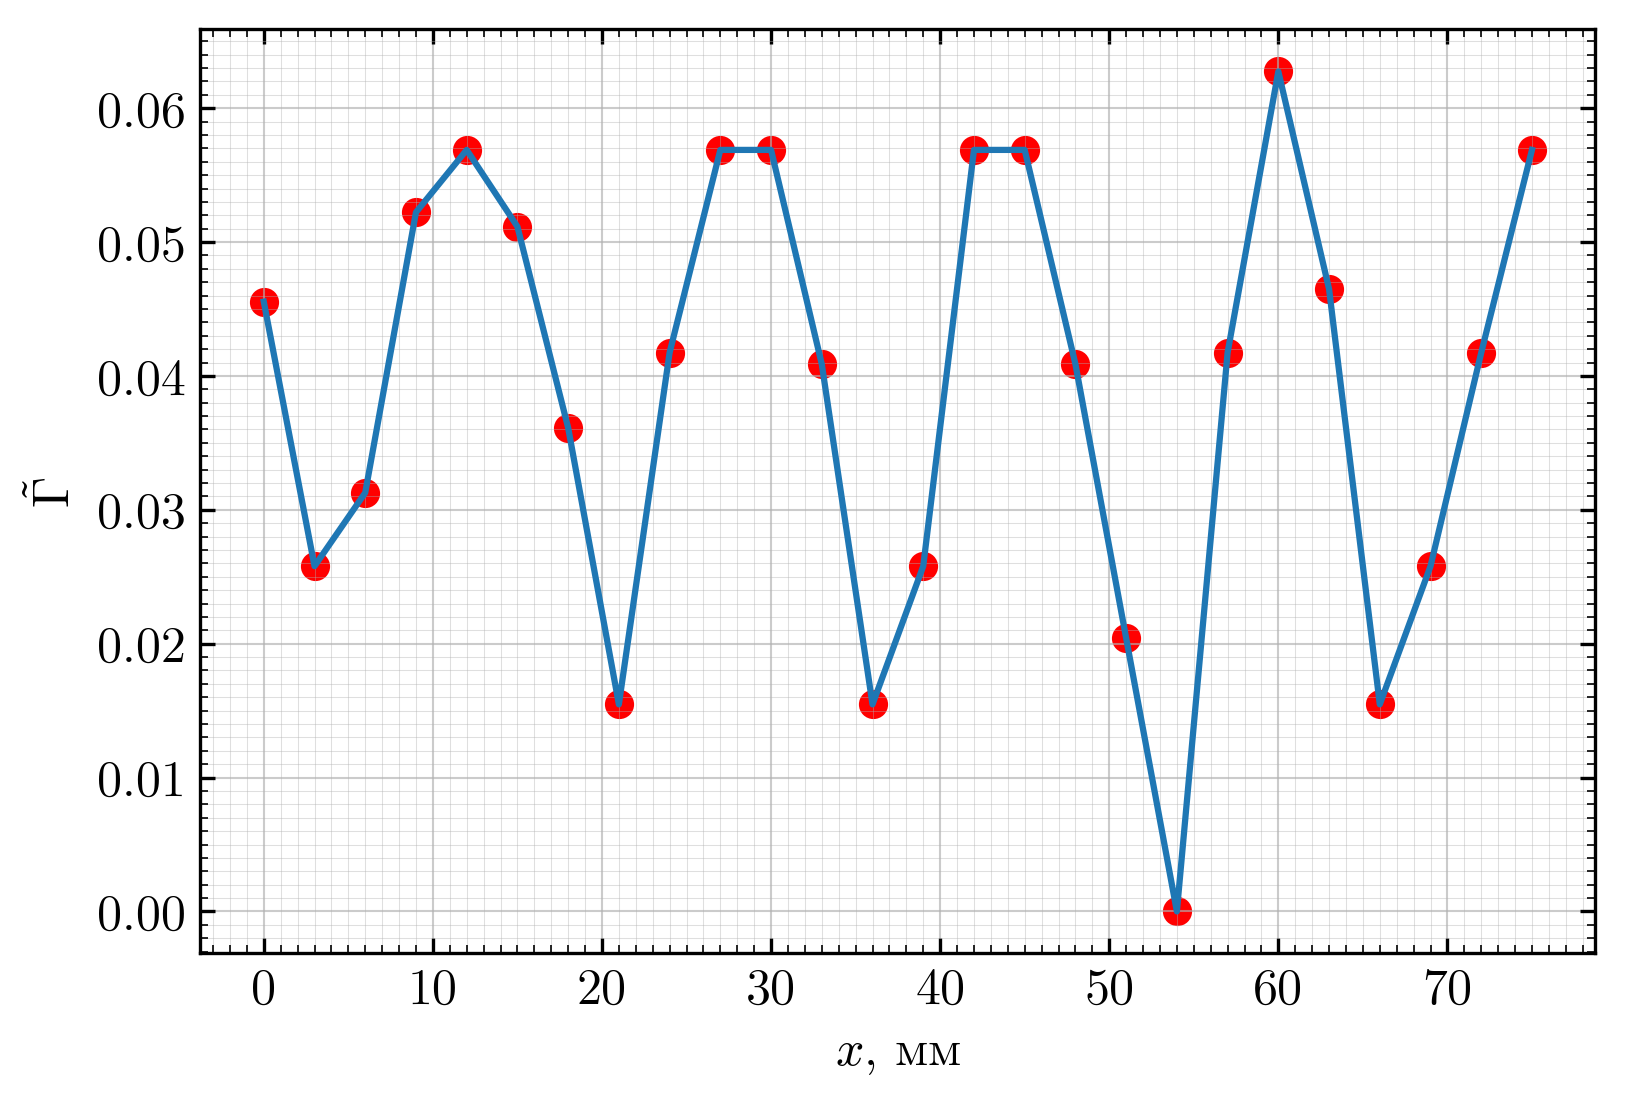
\includegraphics[width=0.7\linewidth]{graph/Figure_3}
	\caption{}
	\label{fig:graph:3}
\end{figure}


Максимум зависимости достигается при
\begin{equation}
	\Delta X = 60~\text{мм},
	\qquad
	\widetilde{\Gamma}_{\max} \approx 0{,}0627.
\end{equation}

Согласно приближённому соотношению
\begin{equation}
	\widetilde{\Gamma}_{\max} \approx \Gamma + \Gamma_{\text{к}},
\end{equation}
получаем
\begin{equation}
	\Gamma_3 = \widetilde{\Gamma}_{\max} - \Gamma_{\text{к}}
	= 0{,}0627 - 0{,}0455
	\approx 0{,}0172.
\end{equation}
Тогда
\begin{equation}
	D_3 = \frac{8\pi X}{\lambda}\Gamma_3
	= \frac{8\pi \cdot 2{,}83}{0{,}03321} \cdot 0{,}0172
	\approx 36{,}8,
\end{equation}
\begin{equation}
	D_3 \approx 15{,}7~\text{дБ}.
\end{equation}

\noindent\textbf{Проверка условия применимости линейного приближения.}
Ранее мы пренебрегли квадратичными членами $\Gamma_{\text{к}}^2$, $\Gamma_3^2$ и $\Gamma_{\text{к}}\Gamma_3$. Теперь, зная их, можно убедиться в их малости:
\begin{equation}
	\Gamma_{\text{к}}^2 = 0{,}0455^2 \approx 0{,}0021,
\end{equation}
\begin{equation}
	\Gamma_3^2 = 0{,}0172^2 \approx 0{,}0003,
\end{equation}
\begin{equation}
	\Gamma_{\text{к}}\Gamma_3 = 0{,}0455 \cdot 0{,}0172 \approx 0{,}0008.
\end{equation}
Все три величины малы по сравнению с единицей, поэтому принятым в теоретической части приближением можно пользоваться.

%\subsection{Сравнение двух экспериментальных методов}
%
%Для одного и того же расстояния $X = 2{,}83$~м получены оценки
%\begin{equation}
%	D_2 \approx 43{,}7, \qquad D_3 \approx 36{,}8.
%\end{equation}
%Их относительное расхождение, рассчитанное относительно среднего значения, составляет
%\begin{equation}
%	\delta_{\text{мет}} = \frac{|D_2 - D_3|}{(D_2 + D_3)/2} \cdot 100\%
%	= \frac{|43{,}7 - 36{,}8|}{(43{,}7 + 36{,}8)/2} \cdot 100\%
%	= \frac{6{,}9}{40{,}25} \cdot 100\%
%	\approx 17{,}1\%.
%\end{equation}
%
%Эту величину следует рассматривать именно как расхождение двух методов, а не как строгую погрешность измерения: в исходных данных не задана инструментальная погрешность отсчёта индикатора и перемещения антенны. На результат влияют дискретность шага, неточность определения экстремумов, остаточное отражение от установки и приближение, при котором малыми квадратичными членами в выражении для поля пренебрегают.
